%
% 6.006 problem set 2 solutions template
%
\documentclass[12pt,twoside]{article}

\newcommand{\name}{}

\usepackage{amssymb}
\usepackage{amsmath}
\usepackage{graphicx}
\usepackage{latexsym}
\usepackage{times,url}
\usepackage{cprotect}
\usepackage{listings}
\usepackage{graphicx}
\usepackage[table]{xcolor}
\usepackage[letterpaper]{geometry}
\usepackage{tikz-qtree}
\usepackage{enumerate}

\newcommand{\profs}{Instructors: Erik Demaine, Jason Ku, and Justin Solomon}
\newcommand{\subj}{6.006}
\newcommand{\ttt}[1]{{\tt\small #1}}

\definecolor{dkgreen}{rgb}{0,0.6,0}
\definecolor{dkblue}{rgb}{.2,.2,1}
\definecolor{gray}{rgb}{0.5,0.5,0.5}
\definecolor{mauve}{rgb}{0.58,0,0.82}

\lstset{
  language=Python,
  aboveskip=1pc,
  belowskip=1pc,
  basicstyle={\footnotesize\ttfamily},
  numbers=left,
  showstringspaces=false,
  numberstyle={\tiny\color{gray}\ttfamily},
  keywordstyle={\color{dkblue}\ttfamily},
  commentstyle={\color{dkgreen}\ttfamily},
  stringstyle={\color{mauve}\ttfamily},
}

% \lstset{
%   language=Python,
%   aboveskip=1pc,
%   belowskip=1pc,
%   basicstyle={\bf\color{white}\ttfamily},
%   numbers=left,
%   showstringspaces=false,
%   numberstyle={\bf\small\color{lightgray}\ttfamily},
%   keywordstyle={\bf\color{cyan}\ttfamily},
%   commentstyle={\bf\color{green}\ttfamily},
%   stringstyle={\bf\color{mauve}\ttfamily},
% }

\tikzset{
  % every node/.style={minimum width=2em,draw,circle},
  % level 1/.style={sibling distance=2cm},
  level distance=1cm,
  edge from parent/.style=
  {draw,edge from parent path={(\tikzparentnode) -- (\tikzchildnode)}},
}
\usetikzlibrary{shapes}

\newif\ifHideSolutions
\newcommand{\solution}[1]{\color{dkgreen}\textbf{Solution: }#1\color{black}}
\newcommand{\commonmistakes}[1]{{\color{dkblue}\textbf{Common Mistakes: }#1}}
\newcommand{\rubric}[1]{\color{dkgreen}{\bf Rubric:} #1\color{black}}

% \HideSolutionsfalse
% \ifHideSolutions
%   \renewcommand{\solution}[1]{}
%   \renewcommand{\rubric}[1]{}
% \fi

\newlength{\toppush}
\setlength{\toppush}{2\headheight}
\addtolength{\toppush}{\headsep}

\newcommand{\htitle}[2]{\noindent\vspace*{-\toppush}\newline\parbox{\textwidth}
{\textit{Introduction to Algorithms: 6.006}\hfill\name\newline
Massachusetts Institute of Technology \hfill #2\newline
\profs\hfill #1 \\[-3.5ex]\newline
\mbox{}\hrulefill\mbox{}}\vspace*{1ex}\mbox{}\newline
\begin{center}{\Large\bf #1}\end{center}}

\newcommand{\handout}[2]{\thispagestyle{empty}
 \markboth{#1}{#1}
 \pagestyle{myheadings}\htitle{#1}{#2}}

\newcommand{\lecture}[3]{\thispagestyle{empty}
 \markboth{Lecture #1: #2}{Lecture #1: #2}
 \pagestyle{myheadings}\htitle{Lecture #1: #2}{#3}}

\newcommand{\htitlewithouttitle}[2]{\noindent\vspace*{-\toppush}\newline\parbox{6.5in}
{\textit{Introduction to Algorithms}\hfill#2\newline
Massachusetts Institute of Technology \hfill 6.006\newline
\profs\hfill Handout #1\vspace*{-.5ex}\newline
\mbox{}\hrulefill\mbox{}}\vspace*{1ex}\mbox{}\newline}

\newcommand{\handoutwithouttitle}[2]{\thispagestyle{empty}
 \markboth{Handout \protect\ref{#1}}{Handout \protect\ref{#1}}
 \pagestyle{myheadings}\htitlewithouttitle{\protect\ref{#1}}{#2}}

\newcommand{\exam}[2]{% parameters: exam name, date
 \thispagestyle{empty}
 \markboth{\hspace{1cm}\subj\ #1\hspace{1in}Name\hrulefill\ \ }%
          {\subj\ #1\hspace{1in}Name\hrulefill\ \ }
 \pagestyle{myheadings}\examtitle{#1}{#2}
 \renewcommand{\theproblem}{Problem \arabic{problemnum}}
}
\newcommand{\examsolutions}[3]{% parameters: handout, exam name, date
 \thispagestyle{empty}
 \markboth{Handout \protect\ref{#1}: #2}{Handout \protect\ref{#1}: #2}
% \pagestyle{myheadings}\htitle{\protect\ref{#1}}{#2}{#3}
 \pagestyle{myheadings}\examsolutionstitle{\protect\ref{#1}} {#2}{#3}
 \renewcommand{\theproblem}{Problem \arabic{problemnum}}
}
\newcommand{\examsolutionstitle}[3]{\noindent\vspace*{-\toppush}\newline\parbox{6.5in}
{\textit{Introduction to Algorithms}\hfill#3\newline
Massachusetts Institute of Technology \hfill 6.006\newline
%Singapore-MIT Alliance \hfill SMA5503\newline
\profs\hfill Handout #1\vspace*{-.5ex}\newline
\mbox{}\hrulefill\mbox{}}\vspace*{1ex}\mbox{}\newline
\begin{center}{\Large\bf #2}\end{center}}

\newcommand{\takehomeexam}[2]{% parameters: exam name, date
 \thispagestyle{empty}
 \markboth{\subj\ #1\hfill}{\subj\ #1\hfill}
 \pagestyle{myheadings}\examtitle{#1}{#2}
 \renewcommand{\theproblem}{Problem \arabic{problemnum}}
}

\makeatletter
\newcommand{\exambooklet}[2]{% parameters: exam name, date
 \thispagestyle{empty}
 \markboth{\subj\ #1}{\subj\ #1}
 \pagestyle{myheadings}\examtitle{#1}{#2}
 \renewcommand{\theproblem}{Problem \arabic{problemnum}}
 \renewcommand{\problem}{\newpage
 \item \let\@currentlabel=\theproblem
 \markboth{\subj\ #1, \theproblem}{\subj\ #1, \theproblem}}
}
\makeatother


\newcommand{\examtitle}[2]{\noindent\vspace*{-\toppush}\newline\parbox{6.5in}
{\textit{Introduction to Algorithms}\hfill#2\newline
Massachusetts Institute of Technology \hfill 6.006 Spring 2020\newline
%Singapore-MIT Alliance \hfill SMA5503\newline
\profs\hfill #1\vspace*{-.5ex}\newline
\mbox{}\hrulefill\mbox{}}\vspace*{1ex}\mbox{}\newline
\begin{center}{\Large\bf #1}\end{center}}

\newcommand{\grader}[1]{\hspace{1cm}\textsf{\textbf{#1}}\hspace{1cm}}

\newcommand{\points}[1]{[#1 points]\ }
\newcommand{\parts}[1]
{
  \ifnum#1=1
  (1 part)
  \else
  (#1 parts)
  \fi
  \ 
}

\newcommand{\bparts}{\begin{problemparts}}
\newcommand{\eparts}{\end{problemparts}}
\newcommand{\ppart}{\problempart}

%\newcommand{\lg} {lg\ }

\setlength{\oddsidemargin}{0pt}
\setlength{\evensidemargin}{0pt}
\setlength{\textwidth}{6.5in}
\setlength{\topmargin}{0in}
\setlength{\textheight}{8.5in}


\newcommand{\Spawn}{{\bf spawn} }
\newcommand{\Sync}{{\bf sync}}

\renewcommand{\cases}[1]{\left\{ \begin{array}{ll}#1\end{array}\right.}
\newcommand{\cif}[1]{\mbox{if $#1$}}
\newcommand{\cwhen}[1]{\mbox{when $#1$}}

\newcounter{problemnum}
\newcommand{\theproblem}{Problem \theproblemsetnum-\arabic{problemnum}}
\newenvironment{problems}{
        \begin{list}{{\bf \theproblem. \hspace*{0.5em}}}
        {\setlength{\leftmargin}{0em}
         \setlength{\rightmargin}{0em}
         \setlength{\labelwidth}{0em}
         \setlength{\labelsep}{0em}
         \usecounter{problemnum}}}{\end{list}}
\makeatletter
\newcommand{\problem}[1][{}]{\item \let\@currentlabel=\theproblem \textbf{#1}}
\makeatother

\newcounter{problempartnum}[problemnum]
\newenvironment{problemparts}{
        \begin{list}{{\bf (\alph{problempartnum})}}
        {\setlength{\leftmargin}{2.5em}
         \setlength{\rightmargin}{2.5em}
         \setlength{\labelsep}{0.5em}}}{\end{list}}
\newcommand{\problempart}{\addtocounter{problempartnum}{1}\item}

\newenvironment{truefalseproblemparts}{
        \begin{list}{{\bf (\alph{problempartnum})\ \ \ T\ \ F\hfil}}
        {\setlength{\leftmargin}{4.5em}
         \setlength{\rightmargin}{2.5em}
         \setlength{\labelsep}{0.5em}
         \setlength{\labelwidth}{4.5em}}}{\end{list}}

\newcounter{exercisenum}
\newcommand{\theexercise}{Exercise \theproblemsetnum-\arabic{exercisenum}}
\newenvironment{exercises}{
        \begin{list}{{\bf \theexercise. \hspace*{0.5em}}}
        {\setlength{\leftmargin}{0em}
         \setlength{\rightmargin}{0em}
         \setlength{\labelwidth}{0em}
         \setlength{\labelsep}{0em}
        \usecounter{exercisenum}}}{\end{list}}
\makeatletter
\newcommand{\exercise}{\item \let\@currentlabel=\theexercise}
\makeatother

\newcounter{exercisepartnum}[exercisenum]
%\newcommand{\problem}[1]{\medskip\mbox{}\newline\noindent{\bf Problem #1.}\hspace*{1em}}
%\newcommand{\exercise}[1]{\medskip\mbox{}\newline\noindent{\bf Exercise #1.}\hspace*{1em}}

\newenvironment{exerciseparts}{
        \begin{list}{{\bf (\alph{exercisepartnum})}}
        {\setlength{\leftmargin}{2.5em}
         \setlength{\rightmargin}{2.5em}
         \setlength{\labelsep}{0.5em}}}{\end{list}}
\newcommand{\exercisepart}{\addtocounter{exercisepartnum}{1}\item}


% Macros to make captions print with small type and 'Figure xx' in bold.
\makeatletter
\def\fnum@figure{{\bf Figure \thefigure}}
\def\fnum@table{{\bf Table \thetable}}
\let\@mycaption\caption
%\long\def\@mycaption#1[#2]#3{\addcontentsline{\csname
%  ext@#1\endcsname}{#1}{\protect\numberline{\csname 
%  the#1\endcsname}{\ignorespaces #2}}\par
%  \begingroup
%    \@parboxrestore
%    \small
%    \@makecaption{\csname fnum@#1\endcsname}{\ignorespaces #3}\par
%  \endgroup}
%\def\mycaption{\refstepcounter\@captype \@dblarg{\@mycaption\@captype}}
%\makeatother
\let\mycaption\caption
%\newcommand{\figcaption}[1]{\mycaption[]{#1}}

\newcounter{totalcaptions}
\newcounter{totalart}

\newcommand{\figcaption}[1]{\addtocounter{totalcaptions}{1}\caption[]{#1}}

% \psfigures determines what to do for figures:
%       0 means just leave vertical space
%       1 means put a vertical rule and the figure name
%       2 means insert the PostScript version of the figure
%       3 means put the figure name flush left or right
\newcommand{\psfigures}{0}
\newcommand{\spacefigures}{\renewcommand{\psfigures}{0}}
\newcommand{\rulefigures}{\renewcommand{\psfigures}{1}}
\newcommand{\macfigures}{\renewcommand{\psfigures}{2}}
\newcommand{\namefigures}{\renewcommand{\psfigures}{3}}

\newcommand{\figpart}[1]{{\bf (#1)}\nolinebreak[2]\relax}
\newcommand{\figparts}[2]{{\bf (#1)--(#2)}\nolinebreak[2]\relax}


\macfigures     % STATE

% When calling \figspace, make sure to leave a blank line afterward!!
% \widefigspace is for figures that are more than 28pc wide.
\newlength{\halffigspace} \newlength{\wholefigspace}
\newlength{\figruleheight} \newlength{\figgap}
\newcommand{\setfiglengths}{\ifnum\psfigures=1\setlength{\figruleheight}{\hruleheight}\setlength{\figgap}{1em}\else\setlength{\figruleheight}{0pt}\setlength{\figgap}{0em}\fi}
\newcommand{\figspace}[2]{\ifnum\psfigures=0\leavefigspace{#1}\else%
\setfiglengths%
\setlength{\wholefigspace}{#1}\setlength{\halffigspace}{.5\wholefigspace}%
\rule[-\halffigspace]{\figruleheight}{\wholefigspace}\hspace{\figgap}#2\fi}
\newlength{\widefigspacewidth}
% Make \widefigspace put the figure flush right on the text page.
\newcommand{\widefigspace}[2]{
\ifnum\psfigures=0\leavefigspace{#1}\else%
\setfiglengths%
\setlength{\widefigspacewidth}{28pc}%
\addtolength{\widefigspacewidth}{-\figruleheight}%
\setlength{\wholefigspace}{#1}\setlength{\halffigspace}{.5\wholefigspace}%
\makebox[\widefigspacewidth][r]{#2\hspace{\figgap}}\rule[-\halffigspace]{\figruleheight}{\wholefigspace}\fi}
\newcommand{\leavefigspace}[1]{\setlength{\wholefigspace}{#1}\setlength{\halffigspace}{.5\wholefigspace}\rule[-\halffigspace]{0em}{\wholefigspace}}

% Commands for including figures with macpsfig.
% To use these commands, documentstyle ``macpsfig'' must be specified.
\newlength{\macfigfill}
\makeatother
\newlength{\bbx}
\newlength{\bby}
\newcommand{\macfigure}[5]{\addtocounter{totalart}{1}
\ifnum\psfigures=2%
\setlength{\bbx}{#2}\addtolength{\bbx}{#4}%
\setlength{\bby}{#3}\addtolength{\bby}{#5}%
\begin{flushleft}
\ifdim#4>28pc\setlength{\macfigfill}{#4}\addtolength{\macfigfill}{-28pc}\hspace*{-\macfigfill}\fi%
\mbox{\psfig{figure=./#1.ps,%
bbllx=#2,bblly=#3,bburx=\bbx,bbury=\bby}}
\end{flushleft}%
\else\ifdim#4>28pc\widefigspace{#5}{#1}\else\figspace{#5}{#1}\fi\fi}
\makeatletter

\newlength{\savearraycolsep}
\newcommand{\narrowarray}[1]{\setlength{\savearraycolsep}{\arraycolsep}\setlength{\arraycolsep}{#1\arraycolsep}}
\newcommand{\normalarray}{\setlength{\arraycolsep}{\savearraycolsep}}

\newcommand{\hint}{{\bf Hint:\ }}

% Macros from /th/u/clr/mac.tex

\newcommand{\set}[1]{\left\{ #1 \right\}}
\newcommand{\abs}[1]{\left| #1\right|}
\newcommand{\card}[1]{\left| #1\right|}
\newcommand{\floor}[1]{\left\lfloor #1 \right\rfloor}
\newcommand{\ceil}[1]{\left\lceil #1 \right\rceil}
\newcommand{\ang}[1]{\ifmmode{\left\langle #1 \right\rangle}
   \else{$\left\langle${#1}$\right\rangle$}\fi}
        % the \if allows use outside mathmode,
        % but will swallow following space there!
\newcommand{\paren}[1]{\left( #1 \right)}
\newcommand{\bracket}[1]{\left[ #1 \right]}
\newcommand{\prob}[1]{\Pr\left\{ #1 \right\}}
\newcommand{\Var}{\mathop{\rm Var}\nolimits}
\newcommand{\expect}[1]{{\rm E}\left[ #1 \right]}
\newcommand{\expectsq}[1]{{\rm E}^2\left[ #1 \right]}
\newcommand{\variance}[1]{{\rm Var}\left[ #1 \right]}
\renewcommand{\choose}[2]{{{#1}\atopwithdelims(){#2}}}
\def\pmod#1{\allowbreak\mkern12mu({\rm mod}\,\,#1)}
\newcommand{\matx}[2]{\left(\begin{array}{*{#1}{c}}#2\end{array}\right)}
\newcommand{\Adj}{\mathop{\rm Adj}\nolimits}

\newtheorem{theorem}{Theorem}
\newtheorem{lemma}[theorem]{Lemma}
\newtheorem{corollary}[theorem]{Corollary}
\newtheorem{xample}{Example}
\newtheorem{definition}{Definition}
\newenvironment{example}{\begin{xample}\rm}{\end{xample}}
\newcommand{\proof}{\noindent{\em Proof.}\hspace{1em}}
\def\squarebox#1{\hbox to #1{\hfill\vbox to #1{\vfill}}}
\newcommand{\qedbox}{\vbox{\hrule\hbox{\vrule\squarebox{.667em}\vrule}\hrule}}
\newcommand{\qed}{\nopagebreak\mbox{}\hfill\qedbox\smallskip}
\newcommand{\eqnref}[1]{(\protect\ref{#1})}

%%\newcommand{\twodots}{\mathinner{\ldotp\ldotp}}
\newcommand{\transpose}{^{\mbox{\scriptsize \sf T}}}
\newcommand{\amortized}[1]{\widehat{#1}}

\newcommand{\punt}[1]{}

%%% command for putting definitions into boldface
% New style for defined terms, as of 2/23/88, redefined by THC.
\newcommand{\defn}[1]{{\boldmath\textit{\textbf{#1}}}}
\newcommand{\defi}[1]{{\textit{\textbf{#1\/}}}}

\newcommand{\red}{\leq_{\rm P}}
\newcommand{\lang}[1]{%
\ifmmode\mathord{\mathcode`-="702D\rm#1\mathcode`\-="2200}\else{\rm#1}\fi}

%\newcommand{\ckt}[1]{\ifmmode\mathord{\mathcode`-="702D\sc #1\mathcode`\-="2200}\else$\mathord{\mathcode`-="702D\sc #1\mathcode`\-="2200}$\fi}
\newcommand{\ckt}[1]{\ifmmode \sc #1\else$\sc #1$\fi}

%% Margin notes - use \notesfalse to turn off notes.
\setlength{\marginparwidth}{0.6in}
\reversemarginpar
\newif\ifnotes
\notestrue
\newcommand{\longnote}[1]{
  \ifnotes
    {\medskip\noindent Note: \marginpar[\hfill$\Longrightarrow$]
      {$\Longleftarrow$}{#1}\medskip}
  \fi}
\newcommand{\note}[1]{
  \ifnotes
    {\marginpar{\tiny \raggedright{#1}}}
  \fi}


\newcommand{\reals}{\mathbbm{R}}
\newcommand{\integers}{\mathbbm{Z}}
\newcommand{\naturals}{\mathbbm{N}}
\newcommand{\rationals}{\mathbbm{Q}}
\newcommand{\complex}{\mathbbm{C}}

\newcommand{\oldreals}{{\bf R}}
\newcommand{\oldintegers}{{\bf Z}}
\newcommand{\oldnaturals}{{\bf N}}
\newcommand{\oldrationals}{{\bf Q}}
\newcommand{\oldcomplex}{{\bf C}}

\newcommand{\w}{\omega}                 %% for fft chapter

\newenvironment{closeitemize}{\begin{list}
{$\bullet$}
{\setlength{\itemsep}{-0.2\baselineskip}
\setlength{\topsep}{0.2\baselineskip}
\setlength{\parskip}{0pt}}}
{\end{list}}

% These are necessary within a {problems} environment in order to restore
% the default separation between bullets and items.
\newenvironment{normalitemize}{\setlength{\labelsep}{0.5em}\begin{itemize}}
                              {\end{itemize}}
\newenvironment{normalenumerate}{\setlength{\labelsep}{0.5em}\begin{enumerate}}
                                {\end{enumerate}}

%\def\eqref#1{Equation~(\ref{eq:#1})}
%\newcommand{\eqref}[1]{Equation (\ref{eq:#1})}
\newcommand{\eqreftwo}[2]{Equations (\ref{eq:#1}) and~(\ref{eq:#2})}
\newcommand{\ineqref}[1]{Inequality~(\ref{ineq:#1})}
\newcommand{\ineqreftwo}[2]{Inequalities (\ref{ineq:#1}) and~(\ref{ineq:#2})}

\newcommand{\figref}[1]{Figure~\ref{fig:#1}}
\newcommand{\figreftwo}[2]{Figures \ref{fig:#1} and~\ref{fig:#2}}

\newcommand{\liref}[1]{line~\ref{li:#1}}
\newcommand{\Liref}[1]{Line~\ref{li:#1}}
\newcommand{\lirefs}[2]{lines \ref{li:#1}--\ref{li:#2}}
\newcommand{\Lirefs}[2]{Lines \ref{li:#1}--\ref{li:#2}}
\newcommand{\lireftwo}[2]{lines \ref{li:#1} and~\ref{li:#2}}
\newcommand{\lirefthree}[3]{lines \ref{li:#1}, \ref{li:#2}, and~\ref{li:#3}}

\newcommand{\lemlabel}[1]{\label{lem:#1}}
\newcommand{\lemref}[1]{Lemma~\ref{lem:#1}} 

\newcommand{\exref}[1]{Exercise~\ref{ex:#1}}

\newcommand{\handref}[1]{Handout~\ref{#1}}

\newcommand{\defref}[1]{Definition~\ref{def:#1}}

% (1997.8.16: Victor Luchangco)
% Modified \hlabel to only get date and to use handouts counter for number.
%   New \handout and \handoutwithouttitle commands in newmac.tex use this.
%   The date is referenced by <label>-date.
%   (Retained old definition as \hlabelold.)
%   Defined \hforcelabel to use an argument instead of the handouts counter.

\newcounter{handouts}
\setcounter{handouts}{0}

\newcommand{\hlabel}[2]{%
\stepcounter{handouts}
{\edef\next{\write\@auxout{\string\newlabel{#1}{{\arabic{handouts}}{0}}}}\next}
\write\@auxout{\string\newlabel{#1-date}{{#2}{0}}}
}

\newcommand{\hforcelabel}[3]{%          Does not step handouts counter.
\write\@auxout{\string\newlabel{#1}{{#2}{0}}}
\write\@auxout{\string\newlabel{#1-date}{{#3}{0}}}}


% less ugly underscore
% --juang, 2008 oct 05
\renewcommand{\_}{\vrule height 0 pt depth 0.4 pt width 0.5 em \,}

% multiline framed box (will always extend to the far right edge; for a short single line, use \fbox directly)
% --zabel, fall 2018
\newcommand\framepar[1]{\fbox{\begin{minipage}{\linewidth}#1\end{minipage}}}


\newcommand{\theproblemsetnum}{2}

\title{6.006 Problem Set 2}

\begin{document}

\handout{Problem Set \theproblemsetnum}

\setlength{\parindent}{0pt}
\medskip\hrulefill\medskip

{\bf Name:} Gabriel Chiong

\medskip

{\bf Collaborators:} None

\medskip\hrulefill

%%%%%%%%%%%%%%%%%%%%%%%%%%%%%%%%%%%%%%%%%%%%%%%%%%%%%
% See below for common and useful latex constructs. %
%%%%%%%%%%%%%%%%%%%%%%%%%%%%%%%%%%%%%%%%%%%%%%%%%%%%%

% Some useful commands:
%$f(x) = \Theta(x)$
%$T(x, y) \leq \log(x) + 2^y + \binom{2n}{n}$
% {\tt code\_function}


% You can create unnumbered lists as follows:
%\begin{itemize}
%    \item First item in a list
%        \begin{itemize}
%            \item First item in a list
%                \begin{itemize}
%                    \item First item in a list
%                    \item Second item in a list
%                \end{itemize}
%            \item Second item in a list
%        \end{itemize}
%    \item Second item in a list
%\end{itemize}

% You can create numbered lists as follows:
%\begin{enumerate}
%    \item First item in a list
%    \item Second item in a list
%    \item Third item in a list
%\end{enumerate}

% You can write aligned equations as follows:
%\begin{align}
%    \begin{split}
%        (x+y)^3 &= (x+y)^2(x+y) \\
%                &= (x^2+2xy+y^2)(x+y) \\
%                &= (x^3+2x^2y+xy^2) + (x^2y+2xy^2+y^3) \\
%                &= x^3+3x^2y+3xy^2+y^3
%    \end{split}
%\end{align}

% You can create grids/matrices as follows:
%\begin{align}
%    A =
%    \begin{bmatrix}
%        A_{11} & A_{21} \\
%        A_{21} & A_{22}
%    \end{bmatrix}
%\end{align}

% You can include images and PDFs as follows:
% 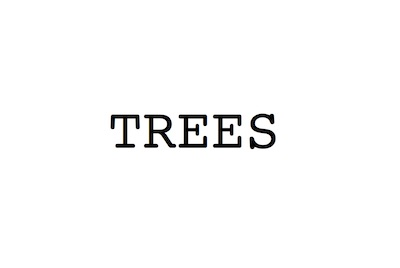
\includegraphics[width=0.5\textwidth]{img.jpg}

\begin{problems}

\problem  % Problem 1

\begin{problemparts}
\problempart % Problem 1a
% An example of embedding images, in case you want to include a drawing of a tree.
% \begin{center}
%   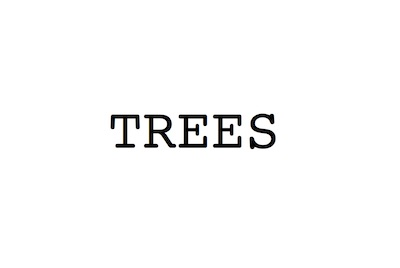
\includegraphics[width=0.5\textwidth]{img.jpg}
% \end{center}
Using the recursion tree method, the tree has depth \(\log_2 n\), with \(4^i \cdot f(\frac{n}{2^i})\) work being done at each level. Therefore, the total work done is \(\sum_{i=0}^{\log_2 n} 4^i \cdot c \frac{n}{2^i} = cn\left(\frac{1-2^{log_2 n + 1}}{1-2}\right)\) by the identity for a geometric series. This simplifies to \(-cn(1-(n+1))=cn^2=O(n^2)\).

Using the Master Theorem, we have \(\log_b a = \log_2 4 = 2\), and \(f(n) = n^{\log_2 4 - 1}\) where \(\varepsilon=1\). Therefore, we are in Case 1 and \(T(n) = O(n^2)\).

\problempart % Problem 1b
Using the recursion tree method, the tree has depth \(\log_{\sqrt{2}}n=2\log_2 n\). At each level, the work done is \(3^i \cdot c\left(\frac{n}{2^{i/2}}\right)^4=cn^4 \cdot \left(\frac{3}{4}\right)^i\). Therefore, the total work done is \(\sum_{i=0}^{2\log_2 n} cn^4 \cdot \left(\frac{3}{4}\right)^i < cn^4 \sum_{i=0}^\infty \left(\frac{3}{4}\right)^i=\frac{cn^4}{1-3/4}=4cn^4=O(n^4)\). 

Using the Master Theorem, we have \(\log_b a = \log_{\sqrt{2}} 3 = 2\log_2 3\). This is less than 4. Therefore, we have \(f(n)=n^4 = n^{\log_{\sqrt{2}} 3 + \varepsilon}\), where \(\varepsilon=4-\log_{\sqrt{2}}3\). We are in Case 3 and \(T(n)=O(n^4)\).

\problempart % Problem 1c
Using the recursion tree method, the tree has depth \(\log_2 n\). At each level, the work done is \(2^i \cdot 5\left(\frac{n}{2^i}\right) \log \left(\frac{n}{2^i}\right)\). Therefore, the total work done is \(\sum_{i=0}^{\log_2n} 2^i \cdot \frac{5n}{2^i} (\log n - \log 2^i)=5n\left(\sum_{i=0}^{\log_2n}\log n - \sum_{i=0}^{\log_2n}i\right)=5n\left(\log^2n-\frac{(\log n + 1)\log n}{2}\right)\), by the summation identity. This can be eventually simplified to \(\frac{5n}{2}\log^2n-\frac{5n}{2}\log n = \Theta(n\log^2 n)\).

Using the Master Theorem, we have \(\log_b a = \log_2 2 = 1\), and \(f(n)=5n\log n\) which matches Case 2: \(f(n)=\Theta(5n^{\log_2 2} \log^k n)=\Theta(n \log^2 n)\). By choosing \(k=1\), we obtain the solution \(T(n)=\Theta(n \log^2 n)\).

\problempart % Problem 1d
We guess that the solution to the recurrence is \(cn^2\). We then rearrange the equation 
\begin{align*}
    \begin{split}
        cn^2 &= c(n-2)^2 + \Theta(n) \\
        cn^2 &= cn^2 - 4cn + 4c + \Theta(n) \\
        \Theta(n) &= 4cn - 4c
    \end{split}
\end{align*}

which is true, therefore we know that the solution is \(\Theta(n^2)\).

\end{problemparts}

\newpage
\problem  % Problem 2

\begin{problemparts}
\problempart % Problem 2a
An in-place sorting algorithm rules out using merge sort. Using insertion sort requires \(O(n^2)\) number of \verb|get_at(i)| operations, and \(O(n^2)\) number of \verb|set_at(i, x)| operations for repeated swaps. Therefore, the overall runtime of using insertion sort is \(O(n^3\log n\) in the worst-case.

Using selection sort results in \(O(n^2)\) number of \verb|get_at(i)| operations, and \(O(n)\) number of \verb|set_at(i, x)| number of operations, since we swap once per iteration. This results in an overall runtime of \(O(n^2\log n)\) in the worst-case using insertion sort.

Therefore, we choose selection sort in this case.

\problempart % Problem 2b
There is no requirement for in-place sorting, so merge sort can be used with a worst-case \(O(n\log n)\) number of comparisons. Both insertion and selection sort require \(O(n^2)\) number of comparisons in the worst-case, which has a poorer performance than merge sort.

\problempart % Problem 2c
Both selection and merge sort take \(\Theta(n^2)\) and \(\Theta(n \log n)\), respectively in the worst-case - regardless of inputs.

However, insertion sort can break its loop early, so it could take \(O(n)\) time for certain inputs. For \(k\) inverted pairs (or pairs that are out of order), insertion sort takes \(O(n+k)\) time. Since \(k=\log \log n\), insertion sort runs in \(O(n + \log \log n) = O(n)\) time. Therefore, we choose insertion sort in this case.

\end{problemparts}

\newpage
\problem  % Problem 3
One possible solution is to search in exponential steps, alternating between \(2^i\) and \(n-2^i\) for \(i=1,2,\ldots,n-2,n-1\). Once the device indicates that the \(2^j\)-th step is too far south or the \(n-2^j\)-th step is too far north, we have identified that either \(2^{j-1}<k<2^j\) or \(n-2^j<k<n-2^{j-1}\). Identifying the correct interval takes \(O(j)\) time in the worst-case.

Applying binary search to the remaining interval of \(2^{j-1}\) takes \(O(\log 2^{j-1})=O(j)\) time in the worst-case. Since we have \(2^{j-1}<k<2^j\) (or equivalently, \(n-2^j<k<n-2^{j-1}\)), then taking the \(\log\) of the statement yields: \(j-1<\log k<j\), which implies \(j=O(\log k)\) as desired.

The algorithm is correct since the first step will identify the bounded range of Datum, and the second step is correct by using binary search on the correctly identified intervals.

\newpage
\problem  % Problem 4
The database can be implemented using a doubly-linked list \(L\) of messages sorted in chronological order, with the most recent ones at the head of the list, as well as a static array \(S\) which contain tuples of a user's id, and a singly-linked list of pointers to the user's messages in \(L\).

To implement \verb|build(V)|, initialize \(L\) to an empty list in \(O(1)\) time, and \(S\) to contain all \(n=|V|\) users in \(O(n)\) time. \verb|None| pointers can be used to signify banned users. To maintain the sorted order of \(S\) by user id, apply merge sort in \(O(n \log n)\) time. Therefore, the overall worst-case time of the \verb|build(V)| operation is \(O(n\log n)\). This is correct as it maintains the invariant of the database.

To implement \verb|send(v, m)|, append the message to \(L\)'s head in \(O(1)\) time. Use binary search to identify the user in \(S\) since it is in sorted order, and append a pointer to the message in \(L\) in \(O(1)\) time (the head of the user's pointer list in \(S\)). This takes \(O(\log n)\) time in the worst-case, and is correct as it maintains the database invariant.

To implement \verb|recent(k)|, simply traverse through \(L\) and return items until either the end of \(L\) is reached, or \(k\) elements have been returned. This takes \(O(k)\) time in the worst case, and is correct by the database invariant.

To implement \verb|ban(v)|, search for the viewer in \(S\) using binary search in \(O(\log n)\) time. Then traverse through the user's messages list and delete each of the messages from \(L\) (and also re-linking adjacent nodes) in \(O(1)\) time. If there are \(n_v\) items in the user's pointer list in \(S\), then the total time to delete from both lists is \(O(n_v)\), since each delete takes \(O(1)\) time in the worst-case. Therefore, the total operation will take \(O(\log n + n_v)\) time, and is correct as in maintains the database invariant.

\newpage
\problem  % Problem 5

\begin{problemparts}
\problempart % Problem 5a
One possible way to solve this is to define two variables, time \(x\) and an empty schedule \(B\). At each time step \(x\), we maintain the invariant that \(B\) is a satisfying booking for \(R_1 \cup R_2\) up to time \(x\). As long as this invariant is maintained, the algorithm will be correct. At initialization (\(x=0\)), this is trivially true since time is nonnegative. If the invariant is true every time \(x\) is increased, once \(x\) increases past the latest finishing time of all requests and the algorithm terminates, \(B\) will contain a satisfying schedule for \(R_1 \cup R_2\).

We maintain two pointers, \(i_1, i_2\) which index the earliest booking under consideration in \(B_1, B_2\) respectively, and repeatedly increase \(x\) until both \(B_1\) and \(B_2\) are depleted.

The algorithm can branch five ways, on each iteration of \(x\):
\begin{itemize}
    \item Case 1: One schedule is depleted. In this case, take the next \((k, \max(x, s), t)\) and append it to \(B\). Set \(x=t\) and increment the index of the schedule that was taken.
    \item Case 2: Neither schedule has been depleted.
        \begin{itemize}
            \item Case 2.1: No booking overlaps with \(x\). Set \(x=\min(s_1, s_2)\) (the minimum start time of either booking). 
            \item Case 2.2: Next booking does not overlap the other after time \(x\). Then we can take this booking \((k, x, t)\) and append it to \(B\), and set \(x=t\). Increase the index of the schedule taken.
            \item Case 2.3: Next booking overlaps with the other after time \(x\). Append the non-overlapping part \((k, s_1, s_2)\) to \(B\) and set \(x=s_2\).
            \item Case 2.4: Both bookings overlap from time \(x\) until \(t^*=\min(t_1, t_2)\). Append the overlapping part \((k_1 + k_2, x, t^*)\) to \(B\) and set \(x=t^*\). Then increase the schedule index that ended at \(t^*\).
        \end{itemize}
\end{itemize}

Since the invariant is maintained on each iteration of the loop, when the algorithm terminates, \(B\) is a satisfying booking for \(R_1 \cup R_2\). Each branch of the loop is executed in \(O(1)\) time, and \(x\) strictly increases, therefore the overall worst-case time complexity is \(O(n)\).

In the final step, we loop through \(B\) and merge adjacent bookings with equal number of rooms, \(k\) in \(O(n)\) time.

\problempart % Problem 5b
We can use a solution similar to merge sort, with the answer to part (a) acting as the "merge" step. Recursively divide \(R\) into roughly equal halves until one element remains, then call the procedure in part (a) on pairs of subproblems to eventually merge them into the final sorted \(B\). At the base case when \(|R|=1\), we return \((1, s, t)\) in \(O(1)\) time. 

The recurrence relation obtained from this algorithm is \(T(n)=2T(n/2)+O(n)\). By the Master Theorem, this falls into Case 2, therefore the algorithm runs in \(O(n \log n)\) time.

\problempart Submit your implementation to {\small\url{alg.mit.edu}}.
\end{problemparts}

\end{problems}

\end{document}
